\documentclass{report}
\usepackage{times}
\usepackage{epsfig}
\usepackage{alltt}
\usepackage{xspace}
\usepackage{graphicx}
\usepackage{ifpdf}
\usepackage{ifthen}
\usepackage{amsmath}
\usepackage{a4wide}

\graphicspath{{figures/}} 

\ifpdf
\DeclareGraphicsExtensions{.pdf, .jpg, .tif, .png}
\else
\DeclareGraphicsExtensions{.eps, .jpg}
\fi

\newboolean{toseecomment}
\setboolean{toseecomment}{false}
%%change to false to hidde comment 
\newcommand{\comment}[1]{\ifthenelse{\boolean{toseecomment}}{$\blacktriangleright$ \textit{#1}$\blacktriangleleft$}{}}

\newcommand{\commented}[1]{}

\newboolean{seevwspecific}
\setboolean{seevwspecific}{true}
\newcommand{\vwspecific}[1]{\ifthenelse{\boolean{seevwspecific}}{#1}{}}

\newboolean{seecategoryspecific}
\setboolean{seecategoryspecific}{false}
\newcommand{\categoryspecific}[1]{\ifthenelse{\boolean{seecategoryspecific}}{#1}{}}

\newboolean{seestorespecific}
\setboolean{seestorespecific}{true}
\newcommand{\storespecific}[1]{\ifthenelse{\boolean{seestorespecific}}{#1}{}}

\newboolean{seesqueakspecific}
\setboolean{seesqueakspecific}{false}
\newcommand{\squeakspecific}[1]{\ifthenelse{\boolean{seesqueakspecific}}{#1}{}}


\newcommand{\category}[0]
{\ifthenelse{\boolean{seestorespecific}}
	{package\xspace}
	{category\xspace}}

\newcommand{\ct}[1]{\texttt{#1}\xspace}
\newcommand{\stc}[1]{{\small {\sf #1}}\xspace}
\newcommand{\ST}{{\textsc Smalltalk}\xspace}
\newcommand{\tab}{\makebox[4em]{}}
\newcommand{\ttt}[1]{{\tt #1}}
\newcommand{\chev}{\ttt{>>}}
\newcommand{\vw}{VisualWorks\xspace}
\newcommand{\sq}{Squeak\xspace}
\newcommand{\store}{Store\xspace}
\renewcommand{\chaptername}{Exercise}
\newcommand{\exercise}{\vspace{0.2cm}\noindent \textbf{Exercise:}\xspace}

\newsavebox{\fminibox}
\newlength{\fminilength}

% Fait un truc encadre
\newenvironment{fminipage}[1][\linewidth]
  {\setlength{\fminilength}{#1-2\fboxsep-2\fboxrule}
        \begin{lrbox}{\fminibox}\begin{minipage}{\fminilength}}
  { \end{minipage}\end{lrbox}\noindent\fbox{\usebox{\fminibox}}}

% Pareil mais pas encadre (a utiliser pour ne pas couper une fonction

\newenvironment{nminipage}[1][\linewidth]
  {\setlength{\fminilength}{#1}
        \begin{lrbox}{\fminibox}\begin{minipage}{\fminilength}}
  { \end{minipage}\end{lrbox}\noindent\mbox{\usebox{\fminibox}}}

% Un alltt encadre
\newenvironment{falltt}
  {\vspace*{0.3cm}\begin{fminipage}\begin{alltt}}
  {\end{alltt}\end{fminipage}\vspace*{0.3cm}}

% Un alltt pas encadre
\newenvironment{nalltt}
  {\vspace*{0.3cm}\begin{nminipage}\begin{alltt}}
  {\end{alltt}\end{nminipage}\vspace*{0.3cm}}

% Une fonction encadree
\newenvironment{ffonction}[1]
  {\begin{fonction}[#1]
        \begin{fminipage}
\begin{alltt}
\rule{\linewidth}{0.5pt}}
{\end{alltt}\end{fminipage}\end{fonction}}

\newenvironment{codeonepage}
  {\begin{nminipage}\vspace*{0.2cm}\hrule\vspace*{0.1cm}
\begin{alltt}}
  {\end{alltt} \vspace*{-0.2cm}\hrule \vspace*{0.2cm} \end{nminipage}}

\newenvironment{code}
  {\vspace*{0.1cm}\hrule\vspace*{-0.1cm}\begin{alltt}}
  {\end{alltt}\vspace*{-0.2cm}\hrule \vspace*{0.1cm}}


%%% for separate compilation
\let\wholebook=\relax

\begin{document}
\title{Object-Oriented Programming in Smalltalk}
\author{Gabriela Ar\'evalo, University of Berne \\
Alexandre Bergel, University of Berne  \\
Prof. Dr. St\'ephane Ducasse, Universit\'e de Savoie  \\
Dr. Roel Wuyts, Universit\'e Libre de Bruxelles \\
}
%{\small Software Composition Group, Institut
%f\"{u}r Informatik
%(IAM)} \\
%{\small Universit\"{a}t Bern, Neubr\"{u}ckstrasse 10, CH-3012 Berne,
%Switzerland} \\
%{\small {\tt \{arevalo, bergel, ducasse, lanza, wuyts\}@iam.unibe.ch}}\\
%{\small {\tt
%http://www.iam.unibe.ch/$\sim$scg/Teaching/Smalltalk03/}}}


\maketitle

% $Author: ducasse $
% $Date: 2005/11/06 13:11:22 $
% $Revision: 1.2 $

\ifx\wholebook\relax\else
\documentclass{report}
\usepackage{times}
\usepackage{epsfig}
\usepackage{alltt}
\usepackage{xspace}
\usepackage{graphicx}
\usepackage{ifpdf}
\usepackage{ifthen}
\usepackage{amsmath}
\usepackage{a4wide}

\graphicspath{{figures/}} 

\ifpdf
\DeclareGraphicsExtensions{.pdf, .jpg, .tif, .png}
\else
\DeclareGraphicsExtensions{.eps, .jpg}
\fi

\newboolean{toseecomment}
\setboolean{toseecomment}{false}
%%change to false to hidde comment 
\newcommand{\comment}[1]{\ifthenelse{\boolean{toseecomment}}{$\blacktriangleright$ \textit{#1}$\blacktriangleleft$}{}}

\newcommand{\commented}[1]{}

\newboolean{seevwspecific}
\setboolean{seevwspecific}{true}
\newcommand{\vwspecific}[1]{\ifthenelse{\boolean{seevwspecific}}{#1}{}}

\newboolean{seecategoryspecific}
\setboolean{seecategoryspecific}{false}
\newcommand{\categoryspecific}[1]{\ifthenelse{\boolean{seecategoryspecific}}{#1}{}}

\newboolean{seestorespecific}
\setboolean{seestorespecific}{true}
\newcommand{\storespecific}[1]{\ifthenelse{\boolean{seestorespecific}}{#1}{}}

\newboolean{seesqueakspecific}
\setboolean{seesqueakspecific}{false}
\newcommand{\squeakspecific}[1]{\ifthenelse{\boolean{seesqueakspecific}}{#1}{}}


\newcommand{\category}[0]
{\ifthenelse{\boolean{seestorespecific}}
	{package\xspace}
	{category\xspace}}

\newcommand{\ct}[1]{\texttt{#1}\xspace}
\newcommand{\stc}[1]{{\small {\sf #1}}\xspace}
\newcommand{\ST}{{\textsc Smalltalk}\xspace}
\newcommand{\tab}{\makebox[4em]{}}
\newcommand{\ttt}[1]{{\tt #1}}
\newcommand{\chev}{\ttt{>>}}
\newcommand{\vw}{VisualWorks\xspace}
\newcommand{\sq}{Squeak\xspace}
\newcommand{\store}{Store\xspace}
\renewcommand{\chaptername}{Exercise}
\newcommand{\exercise}{\vspace{0.2cm}\noindent \textbf{Exercise:}\xspace}

\newsavebox{\fminibox}
\newlength{\fminilength}

% Fait un truc encadre
\newenvironment{fminipage}[1][\linewidth]
  {\setlength{\fminilength}{#1-2\fboxsep-2\fboxrule}
        \begin{lrbox}{\fminibox}\begin{minipage}{\fminilength}}
  { \end{minipage}\end{lrbox}\noindent\fbox{\usebox{\fminibox}}}

% Pareil mais pas encadre (a utiliser pour ne pas couper une fonction

\newenvironment{nminipage}[1][\linewidth]
  {\setlength{\fminilength}{#1}
        \begin{lrbox}{\fminibox}\begin{minipage}{\fminilength}}
  { \end{minipage}\end{lrbox}\noindent\mbox{\usebox{\fminibox}}}

% Un alltt encadre
\newenvironment{falltt}
  {\vspace*{0.3cm}\begin{fminipage}\begin{alltt}}
  {\end{alltt}\end{fminipage}\vspace*{0.3cm}}

% Un alltt pas encadre
\newenvironment{nalltt}
  {\vspace*{0.3cm}\begin{nminipage}\begin{alltt}}
  {\end{alltt}\end{nminipage}\vspace*{0.3cm}}

% Une fonction encadree
\newenvironment{ffonction}[1]
  {\begin{fonction}[#1]
        \begin{fminipage}
\begin{alltt}
\rule{\linewidth}{0.5pt}}
{\end{alltt}\end{fminipage}\end{fonction}}

\newenvironment{codeonepage}
  {\begin{nminipage}\vspace*{0.2cm}\hrule\vspace*{0.1cm}
\begin{alltt}}
  {\end{alltt} \vspace*{-0.2cm}\hrule \vspace*{0.2cm} \end{nminipage}}

\newenvironment{code}
  {\vspace*{0.1cm}\hrule\vspace*{-0.1cm}\begin{alltt}}
  {\end{alltt}\vspace*{-0.2cm}\hrule \vspace*{0.1cm}}


\begin{document}
\fi

%%% Log
% ducasse: 6 may 2005 
% uses scode
% fixes some missing \stc uses

\chapter{Smalltalk Environment Basics}

\mainauthor{Ducasse and Wuyts}


\section{Videos}
You can find videos showing some important points of Smalltalk manipulation
at http://www.iam.unibe.ch/~ducasse/Videos/SqueakOriginalMov/.


\section{Starting up}
Similarly to Java, Smalltalk the source code is translated to byte-codes, which are then interpreted and executed by the Smalltalk Virtual Machine. (Note that this is an approximation  because Smalltalk dialects were also the first languages to develop 
Just in Time compilation, \ie  a method is compiled into byte-codes but also into native code that is directly called instead of  executing the byte codes.) 

There are three important  files:

\begin{description}
\item{\vwspecific{\textbf{visual.im}}\squeakspecific{\textbf{Squeak.image}}} (Binary): contains byte code of all the object of the  system, the libraries and the modifications you made.
\item{\vwspecific{\textbf{visual.cha}}\squeakspecific{\textbf{Squeak.changes}}} (ASCII): contains all the modifications made in the image-file since this was created. It contains also all the code of the actions you will perform.
\item{\vwspecific{\textbf{visual.sou}}\squeakspecific{\textbf{SqueakV3.sources}}}  (ASCII): contains the textual code of the initial classes of the system. 
\end{description}

To open an image with drag-drop (on Macintosh, Windows):
\begin{itemize}
\item Drag the file 'visual.im' on the virtual machine to start the image.
\item If  you want to start your own image, just double click on it or drag it over the virtual machine.
\end{itemize}

On Unixes (Linux, Solaris, HPUX, AIX, ...): you should invoke the virtual machine passing it an image as parameter. For the first opening, execute the first script that per default 
uses the original image the script is installation dependent but  should look like path/bin/visualworks path/image/visual.im Then after you can specify your own image. 

\vwspecific{
\section{First Impressions}
After opening the image, and thus starting a Smalltalk session, you see two windows : the launcher (with menu, buttons and a transcript), and a Workspace window (the one containing text). You  can minimize or close this last one, since we do not need it for the  moment.

The launcher is the starting point for working with your environment  and for the opening of all the programming tools that you might need.  To begin, we will first create a fresh image.}

\paragraph{Creating a fresh image.}
We are going to create an image for this lesson. 
\begin{itemize}
\item	select �Save As...� in the menu
\item	when the system prompts you for the name for the new image, you type \emph{lesson}, followed by your username.
\item	the image is saved in the image directory.
\item	Have a look at the Transcript, and note what it says.
\end{itemize}

\vwspecific{
The \stc{Transcript} is the lower part of the Launcher, and gives you 
system messages, like the one you see right now. We will see later on 
how you can put your own messages there.}

\paragraph{About the mouse.}
Smalltalk  was the first application  to use multiple overlapping windows and a mouse. It extensively uses 
three mouse buttons, that are context sensitive and can be used 
everywhere throughout Smalltalk:
\begin{itemize}
\item	the left mouse button is the select button
\item	the middle button is the operate button
\item	the right button is the window button
\end{itemize}

On a Macintosh, where only one button is available, you have to use 
some keyboard keys together with pressing your mouse button:
\begin{itemize}
\item	the select button is the one button itself
\item	for the operate button, press the button while holding the alt-key 
pressed
\item	for the window button, press the button while holding the apple-key 
pressed
\end{itemize}

\section{Adding Goodies and setting Preferences}
Out of the box, there is already quite some code in a Smalltalk image (about 1000 classes containing the basic system: the complete compiler, parser classes, GUI framework, development environment, debugger, collection libraries, etc.) \footnote{To answer a common question: yes, there are ways to strip this so that you can deploy smaller images to clients that do not contain all of these tools.}. But for developing, it is convenient to load some extra tools. 

\vwspecific{
You may have to load a package named \emph{ImageConfiguration} or parcels. To load parcels we can use the \emph{Parcel Manager} application (open it using the System menu in the Launcher). There is lots of optional applications you might load. Use it to load:
\begin{itemize}
	\item \emph{RBSUnitExtentions} (in \emph{Environment Enhancements})
	\item \emph{MagicKeys} (in \emph{Environment Enhancements})
	\item \emph{ColorEditing} (in \emph{Environment Enhancements})
	\item \emph{RB\_Tabs} (in \emph{Environment Enhancements})
\end{itemize}

You can also edit systemwide preferences. To do so, open the \emph{Settings} application, again in the System menu in the Launcher. Use it to set a setting in Tools/Browser: select \emph{Show all methods when no protocols are selected}.}

\sqspecific{Using the open... Squeak Map Package Loader entry, you can load the following tools: Shout, eCompletion, Refactoring Browser. Normally we already loaded them in the image you are using. }

\section{Selecting text, and doing basic text manipulations}
One of the basic manipulations you do when programming is working 
with text. Therefore, this section introduces you to the different 
ways you can select text, and manipulate these selections.

The basic way of selecting text is by clicking in front of the first 
character you want to select, and dragging your mouse to the last 
character you want in the selection while keeping the button pressed 
down. Selected text will be highlighted. 

\exercise Select some parts of text in the Transcript.
You can also select a single word by double clicking on it. When the 
text is delimited by '' (single quotes), "" (double quotes), () 
(parentheses), [] (brackets), or {} (braces), you can select anything 
in between by double clicking just after the first delimiter.

\exercise Try these new selection techniques.

Now have a look at the text operations. Select a piece of text in the 
\stc{Transcript}, and bring on the operate menu. Note that you have to 
keep your mouse button pressed to keep seeing the window. 

\exercise Copy this piece of text, and paste it after your 
selection. Afterwards cut the newly inserted piece of text.

\exercise See if there is an occurrence of the word visual in the 
Transcript. Note that to find things in a text window, there is no 
need to select text. Just bring up the operate menu . 

\exercise Replace the word visual with C++ using the replace 
operation (if it does not contain Smalltalk, add this word or replace 
something else). Take your time and explore the different options of 
the replace operation.

\exercise Bring up the operate menu, but don't select anything yet. 
Press and hold the shift button, and select paste in the operation 
menu. What happens ?

\section{Opening a WorkSpace Window}
We will now open a workspace window, a text window much like the 
\stc{Transcript}, you use to type text and expressions and evaluate them. 

To open a workspace:
\begin{itemize}
\vwspecific{\item	select the tools menu in the Launcher
\item from the tools menu, select Workspace}
\sqspecific{\item open the left flap or bring the world menu and choose open...}
\item	You will see a framing rectangle (with your mouse in the upper left 
corner), that indicates the position where the Workspace will open. 
Before you click, you can move your mouse around to change this 
position. Click one time once you have found a good spot for your 
Workspace. 

\item	Now your mouse is in the bottom right corner, and you can adjust 
the size. If you click once more, once you have given it the size you 
like, the Workspace window appears.
\end{itemize}

This is the basic way of opening many kinds of applications. Experiment with it until you feel comfortable with it.



\section{Evaluating Expressions}
In the Workspace, type : \stc{3}.
Select it, and bring up the operate menu.
In the operate you will see the next three different options for 
evaluating text and getting the result:

\begin{description}
\item[do it:] do it evaluates the current selection, and does not show any 
result of the execution result. 
\item[print it:] prints the result of the execution after your selection. 
The result is automatically highlighted, so you can easily delete it 
if you want to.
\item[inspect it:] opens an inspector on the result of the execution.
\end{description}

The distinction before these three operations is essential, so check 
that you REALLY understand their differences
\exercise Select 3, bring up the operate menu, and select print it.

\exercise Print the result of \stc{3+4}

\exercise Type \stc{Date today} and print it. Afterwards, select it again 
and inspect it.

After exercise 9, you will have an inspector on the result of the 
evaluation of the expression Date today (this tells Smalltalk to 
create an object containing the current date). This Inspector Window 
consists of two parts: the left one is a list view containing self (a 
pseudo variable containing the object you are inspecting) and the 
instance variables of the object. Right is a text field.

\exercise Click on \stc{self} in the inspector. What do you get? Does 
it resemble the result shown by printstring?

\exercise Select \stc{day}. What do you get? Now change this value, 
bring up the operate menu, and select accept it. Click again on 
\stc{self}. 
Any difference? 

\exercise In the inspector edit field, type the following: self 
weekday, select it and print it. This causes the message weekday to 
be sent to self (\ie the date object), and the result is printed. 
Experiment with other expressions like:

\begin{scode}
self daysInMonth
self monthName
\end{scode}

Close the inspector when you are finished.

\exercise	Type in the Workspace the following expression: \ct{Time 
now}, and inspect it. Have a look at self and the instance variables.

\exercise Type in the Workspace the following expression: \stc{Time 
dateAndTimeNow}. This tells the system to create an object 
representing both today's date and the current time, and open an 
inspector on it. Select the item \stc{self} in the inspector. [Note that 
self is an object called an Array. It holds on to two other objects 
(elements 1 and 2). You can inspect each element to get either the 
time or the date object.

\paragraph{Using the System Transcript.} 
We have already seen that the Transcript is a text window  where the system informs you important 
information. You can also use the Transcript yourself as a very cheap 
user interface.

If you have a Workspace open, place it so that it does not cover the 
System Transcript. Otherwise, open one and take care of  where you 
put it. Now, in the Workspace, type:

\begin{scode}
Transcript cr.
Transcript show: 'This is a test'.
Trancript cr.
\end{scode}

Select these 3 lines and evaluate (do It) them with do it.
This will cause the string This is a test to be printed in the 
\stc{Transcript}, preceeded and followed by a carriage return. Note that 
the argument of the show: message was a literal string (you see this 
because it is contained in single quotes). It is important to know, 
because the argument of the show: method always has to be a string. 
This means that if you want any non-string object to be printed (like 
a Number for example), you first have to convert it to a string by 
sending the message \stc{printString} to it. For example, type in the 
workspace the following expression and evaluate it:

\stc{Transcript show: 42 printString, 'is the answer to the Universe'}.
Note here that the comma is used to concatenate the two strings that 
are passed to the \stc{show:} message \stc{42 printString} and \stc{'is the answer to 
the Universe'}.

\exercise Experiment on your own with different expressions.
\stc{Transcript cr ; show: �This is a test� ; cr} Explain why this expression gives the same result that before. What  is the semantics of  �;� ?



\ifx\wholebook\relax\else\end{document}\fi

% $Author: ducasse $
% $Date: 2005/11/06 13:11:22 $
% $Revision: 1.2 $
\ifx\wholebook\relax\else
\documentclass{report}
\usepackage{times}
\usepackage{epsfig}
\usepackage{alltt}
\usepackage{xspace}
\usepackage{graphicx}
\usepackage{ifpdf}
\usepackage{ifthen}
\usepackage{amsmath}
\usepackage{a4wide}

\graphicspath{{figures/}} 

\ifpdf
\DeclareGraphicsExtensions{.pdf, .jpg, .tif, .png}
\else
\DeclareGraphicsExtensions{.eps, .jpg}
\fi

\newboolean{toseecomment}
\setboolean{toseecomment}{false}
%%change to false to hidde comment 
\newcommand{\comment}[1]{\ifthenelse{\boolean{toseecomment}}{$\blacktriangleright$ \textit{#1}$\blacktriangleleft$}{}}

\newcommand{\commented}[1]{}

\newboolean{seevwspecific}
\setboolean{seevwspecific}{true}
\newcommand{\vwspecific}[1]{\ifthenelse{\boolean{seevwspecific}}{#1}{}}

\newboolean{seecategoryspecific}
\setboolean{seecategoryspecific}{false}
\newcommand{\categoryspecific}[1]{\ifthenelse{\boolean{seecategoryspecific}}{#1}{}}

\newboolean{seestorespecific}
\setboolean{seestorespecific}{true}
\newcommand{\storespecific}[1]{\ifthenelse{\boolean{seestorespecific}}{#1}{}}

\newboolean{seesqueakspecific}
\setboolean{seesqueakspecific}{false}
\newcommand{\squeakspecific}[1]{\ifthenelse{\boolean{seesqueakspecific}}{#1}{}}


\newcommand{\category}[0]
{\ifthenelse{\boolean{seestorespecific}}
	{package\xspace}
	{category\xspace}}

\newcommand{\ct}[1]{\texttt{#1}\xspace}
\newcommand{\stc}[1]{{\small {\sf #1}}\xspace}
\newcommand{\ST}{{\textsc Smalltalk}\xspace}
\newcommand{\tab}{\makebox[4em]{}}
\newcommand{\ttt}[1]{{\tt #1}}
\newcommand{\chev}{\ttt{>>}}
\newcommand{\vw}{VisualWorks\xspace}
\newcommand{\sq}{Squeak\xspace}
\newcommand{\store}{Store\xspace}
\renewcommand{\chaptername}{Exercise}
\newcommand{\exercise}{\vspace{0.2cm}\noindent \textbf{Exercise:}\xspace}

\newsavebox{\fminibox}
\newlength{\fminilength}

% Fait un truc encadre
\newenvironment{fminipage}[1][\linewidth]
  {\setlength{\fminilength}{#1-2\fboxsep-2\fboxrule}
        \begin{lrbox}{\fminibox}\begin{minipage}{\fminilength}}
  { \end{minipage}\end{lrbox}\noindent\fbox{\usebox{\fminibox}}}

% Pareil mais pas encadre (a utiliser pour ne pas couper une fonction

\newenvironment{nminipage}[1][\linewidth]
  {\setlength{\fminilength}{#1}
        \begin{lrbox}{\fminibox}\begin{minipage}{\fminilength}}
  { \end{minipage}\end{lrbox}\noindent\mbox{\usebox{\fminibox}}}

% Un alltt encadre
\newenvironment{falltt}
  {\vspace*{0.3cm}\begin{fminipage}\begin{alltt}}
  {\end{alltt}\end{fminipage}\vspace*{0.3cm}}

% Un alltt pas encadre
\newenvironment{nalltt}
  {\vspace*{0.3cm}\begin{nminipage}\begin{alltt}}
  {\end{alltt}\end{nminipage}\vspace*{0.3cm}}

% Une fonction encadree
\newenvironment{ffonction}[1]
  {\begin{fonction}[#1]
        \begin{fminipage}
\begin{alltt}
\rule{\linewidth}{0.5pt}}
{\end{alltt}\end{fminipage}\end{fonction}}

\newenvironment{codeonepage}
  {\begin{nminipage}\vspace*{0.2cm}\hrule\vspace*{0.1cm}
\begin{alltt}}
  {\end{alltt} \vspace*{-0.2cm}\hrule \vspace*{0.2cm} \end{nminipage}}

\newenvironment{code}
  {\vspace*{0.1cm}\hrule\vspace*{-0.1cm}\begin{alltt}}
  {\end{alltt}\vspace*{-0.2cm}\hrule \vspace*{0.1cm}}


\begin{document}
\fi


\chapter{Objects and expressions}

This lesson is about reading and understanding Smalltalk
expressions, and differentiating between different types of
messages and receivers. Note that in the expressions you will be
asked to read and evaluate, you can assume that the implementation
of methods generally corresponds to what their message names imply
(\ie \ct{2 + 2 = 4}). \\
\exercise For each of the Smalltalk
expressions below, fill in the answers:

\begin{scode}
3 + 4
\end{scode}

\begin{itemize}
\item What is the receiver object?
\item What is the message selector?
\item What is/are the argument (s)?
\item What is the message?
\item What is the result returned by evaluating this expression?
\end{itemize}

\begin{scode}
Date today
\end{scode}
\begin{itemize}
\item What is the receiver object?
\item What is the message selector?
\item What is/are the argument (s)?
\item What is the message?
\item What is the result returned by evaluating this expression?
\end{itemize}

\begin{scode}
anArray at: 1 put: 'hello'
\end{scode}

\begin{itemize}
\item What is the receiver object?
\item What is the message selector?
\item What is/are the argument (s)?
\item What is the message?
\item What is the result returned by evaluating this expression?
\end{itemize}

\exercise What kind of object does the literal expression \stc{'Hello, Dave'} describe?

\exercise What kind of object does the literal expression \stc{\#Node1} describe?

\exercise What kind of object does the literal expression \stc{\#(1 2 3)} describe?

\exercise What can one assume about a variable named \stc{Transcript}?

\exercise What can one assume about a variable named \stc{rectangle}?

\exercise Examine the following expression:

\begin{scode}
\stBar anArray \stBar
anArray := \#('first' 'second' 'third' 'fourth').
anArray at: 2
\end{scode}

What is the resulting value when it is evaluated (\^{ } means return)?
What happens if you remove the \^{ }. Explain

\exercise Which sets of parentheses are redundant with regard to
evaluation of the following expressions:

\begin{scode}
((3 + 4) + (2 * 2) + (2 * 3))

(x isZero)
   ifTrue: [....]
(x includes: y)
   ifTrue: [....]
\end{scode}

\exercise Guess what are the results of the following expressions

\begin{scode}
6 + 4 / 2
1 + 3 negated
1 + (3 negated)
2 raisedTo: 3 + 2
2 negated raisedTo: 3 + 2
\end{scode}

\exercise Examine the following expression:
\begin{scode}
25@50
\end{scode}

\begin{itemize}
\item What is the receiver object?
\item What is the message selector?
\item What is/are the argument (s)?
\item What is the message?
\item What is the result returned by evaluating this expression?
\end{itemize}

\exercise Examine the following expression and write down the sequence of steps that the Smalltalk system would take to execute the following expression:
\begin{scode}
Date today daysInMonth
\end{scode}
\exercise Examine the following expression and write down the
sequence of steps that the Smalltalk system would take to execute
the following expression:
\begin{scode}
Transcript show: (45 + 9) printString
\end{scode}
\exercise Examine the following expression and write down the
sequence of steps that the Smalltalk system would take to execute
the following expression:
\begin{scode}
5@5 extent: 6.0 truncated @ 7
\end{scode}
\exercise During lecture, we saw how to write strings to the
Transcript, and how the message \stc{printString} could be sent
to any non-string object to obtain a string representation. Now
write a Smalltalk expression to print the result of \stc{34 +
89} on the Transcript. Test your code !

\newpage
\exercise Examine the block expression:

\begin{scode}
\stBar anArray sum \stBar
sum := 0.
anArray := \#(21 23 53 66 87).
anArray do: [:item \stBar sum := sum + item].
sum
\end{scode}

What is the final result of sum ? How could this piece of code be
rewritten to use explicit array indexing (with the method
\stc{at:} ) to access the array elements\footnote{Note this is
how you would proceed with Java or C++}? Test your version.
Rewrite this code using \stc{inject:into:}


\ifx\wholebook\relax\else\end{document}\fi

% $Author: ducasse $
% $Date: 2005/11/06 13:11:22 $
% $Revision: 1.3 $
\ifx\wholebook\relax\else
\documentclass{report}
\usepackage{times}
\usepackage{epsfig}
\usepackage{alltt}
\usepackage{xspace}
\usepackage{graphicx}
\usepackage{ifpdf}
\usepackage{ifthen}
\usepackage{amsmath}
\usepackage{a4wide}

\graphicspath{{figures/}} 

\ifpdf
\DeclareGraphicsExtensions{.pdf, .jpg, .tif, .png}
\else
\DeclareGraphicsExtensions{.eps, .jpg}
\fi

\newboolean{toseecomment}
\setboolean{toseecomment}{false}
%%change to false to hidde comment 
\newcommand{\comment}[1]{\ifthenelse{\boolean{toseecomment}}{$\blacktriangleright$ \textit{#1}$\blacktriangleleft$}{}}

\newcommand{\commented}[1]{}

\newboolean{seevwspecific}
\setboolean{seevwspecific}{true}
\newcommand{\vwspecific}[1]{\ifthenelse{\boolean{seevwspecific}}{#1}{}}

\newboolean{seecategoryspecific}
\setboolean{seecategoryspecific}{false}
\newcommand{\categoryspecific}[1]{\ifthenelse{\boolean{seecategoryspecific}}{#1}{}}

\newboolean{seestorespecific}
\setboolean{seestorespecific}{true}
\newcommand{\storespecific}[1]{\ifthenelse{\boolean{seestorespecific}}{#1}{}}

\newboolean{seesqueakspecific}
\setboolean{seesqueakspecific}{false}
\newcommand{\squeakspecific}[1]{\ifthenelse{\boolean{seesqueakspecific}}{#1}{}}


\newcommand{\category}[0]
{\ifthenelse{\boolean{seestorespecific}}
	{package\xspace}
	{category\xspace}}

\newcommand{\ct}[1]{\texttt{#1}\xspace}
\newcommand{\stc}[1]{{\small {\sf #1}}\xspace}
\newcommand{\ST}{{\textsc Smalltalk}\xspace}
\newcommand{\tab}{\makebox[4em]{}}
\newcommand{\ttt}[1]{{\tt #1}}
\newcommand{\chev}{\ttt{>>}}
\newcommand{\vw}{VisualWorks\xspace}
\newcommand{\sq}{Squeak\xspace}
\newcommand{\store}{Store\xspace}
\renewcommand{\chaptername}{Exercise}
\newcommand{\exercise}{\vspace{0.2cm}\noindent \textbf{Exercise:}\xspace}

\newsavebox{\fminibox}
\newlength{\fminilength}

% Fait un truc encadre
\newenvironment{fminipage}[1][\linewidth]
  {\setlength{\fminilength}{#1-2\fboxsep-2\fboxrule}
        \begin{lrbox}{\fminibox}\begin{minipage}{\fminilength}}
  { \end{minipage}\end{lrbox}\noindent\fbox{\usebox{\fminibox}}}

% Pareil mais pas encadre (a utiliser pour ne pas couper une fonction

\newenvironment{nminipage}[1][\linewidth]
  {\setlength{\fminilength}{#1}
        \begin{lrbox}{\fminibox}\begin{minipage}{\fminilength}}
  { \end{minipage}\end{lrbox}\noindent\mbox{\usebox{\fminibox}}}

% Un alltt encadre
\newenvironment{falltt}
  {\vspace*{0.3cm}\begin{fminipage}\begin{alltt}}
  {\end{alltt}\end{fminipage}\vspace*{0.3cm}}

% Un alltt pas encadre
\newenvironment{nalltt}
  {\vspace*{0.3cm}\begin{nminipage}\begin{alltt}}
  {\end{alltt}\end{nminipage}\vspace*{0.3cm}}

% Une fonction encadree
\newenvironment{ffonction}[1]
  {\begin{fonction}[#1]
        \begin{fminipage}
\begin{alltt}
\rule{\linewidth}{0.5pt}}
{\end{alltt}\end{fminipage}\end{fonction}}

\newenvironment{codeonepage}
  {\begin{nminipage}\vspace*{0.2cm}\hrule\vspace*{0.1cm}
\begin{alltt}}
  {\end{alltt} \vspace*{-0.2cm}\hrule \vspace*{0.2cm} \end{nminipage}}

\newenvironment{code}
  {\vspace*{0.1cm}\hrule\vspace*{-0.1cm}\begin{alltt}}
  {\end{alltt}\vspace*{-0.2cm}\hrule \vspace*{0.1cm}}


\begin{document}
\fi


\chapter{Counter Example}

\mainauthor{Bergel, Ducasse, Wuyts}

\section{A Simple Counter}
We want you to implement a simple counter that follows the small example given
below. Please note that we will ask you to define a test for this example.

\begin{scode}
\stBar counter \stBar
counter := SimpleCounter new.
counter increment; increment.
counter decrement.
counter value = 1
\end{scode}


\section{Creating your own class}
In this part you will create your first class. In traditional Smalltalk environments a class is associated with a category (a folder containing the classes of your project).

\storespecific{When we are using \store, categories are replaced
by packages. Therefore in \vw with \store you define a package and
define your class within this package.} The steps we will do are the same ones every  time you create a class, so memorize them well. We are going to create a class \stc{SimpleCounter} in a
\category called \stc{DemoCounter}. Figure \ref{fig:packageCreated} shows the result of creating such a \category.
\storespecific{Note that you all will be versioning your code in the \store database -with the rest of the students of the lecture-, so every package (each one belonging to different group of students) must have a different name. Therefore you should prefix them with your initials or group name.}

\storespecific{
\subsection{Creating a Package}
In the System Browser, click on the line \stc{Local Image}
located in the left-most upper pane (left button of the mouse) and
select \stc{New}\sepa\stc{Package}. The system will ask you a
name. You should write \stc{DemoCounter}, postfixed with your initials or group name. This new package will be created and added to the list (see Figure~\ref{fig:packageCreated}).

With the package selected, as shown in Figure~\ref{fig:packageCreated}, you can edit its properties by clicking the \stc{properties tab} of the editor. Properties you will likely have to set one day are the dependencies on other packages (for example, when you subclass a class from another package), post-load actions (an expression that is executed after loading that package from Store, for example to initialize something) and pre-unload actions (an expression that is executed just before unloading a package from your image, for example to close any windows from an application). In the context of this exercise we do not need any of this, so leave the properties alone for now.}

\squeakspecific{
\subsection{Creating a Class category}
In the System Browser, click on the left pane and select \emph{add}. The
system will ask you a name. You should write \stc{DemoCounter}.
This new \category will be created and added to the list.}

%\vwspecific{\subsection*{With Namespace} In \vw you can also define your own namespace. If you do so you will have to define your namespace (in the \emph{class} menu of the browser) before you can define the class in this new namespace. For now we suggest you to use the default namespace called \ct{Smalltalk}. Note that classes (or methods or namespaces) can be moved to other namespaces or packages anytime.}

\subsection{Creating a Class}
\storespecific{
\begin{figure}[htbp]
\begin{center}
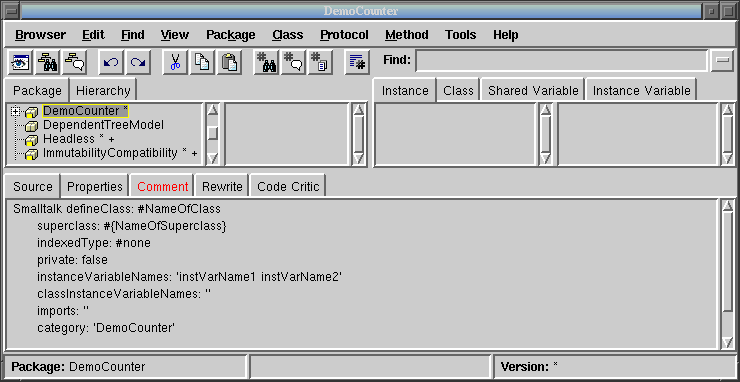
\includegraphics[scale=0.5]{nlesson3Fig4Package}
\caption{Your package is created.} \label{fig:packageCreated}
\end{center}
\end{figure}}

\categoryspecific{
\begin{figure}[htbp]
\begin{center}
\vwspecific{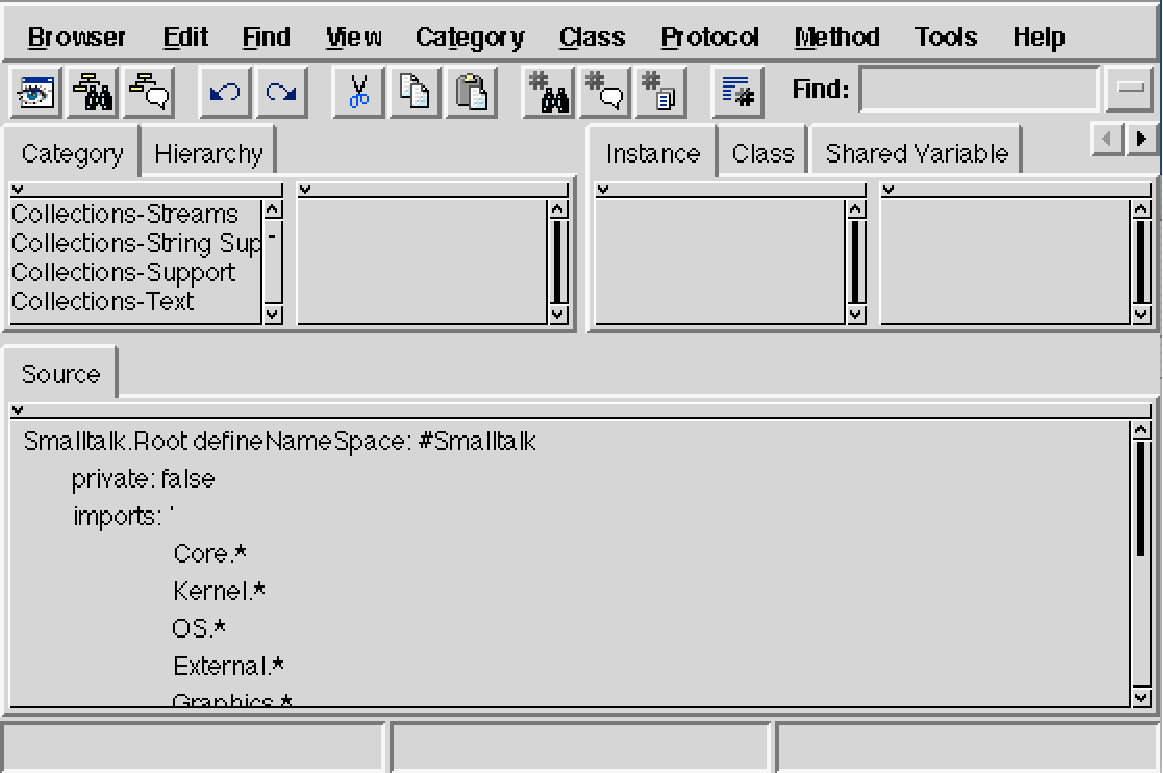
\includegraphics[scale=0.5]{nlesson3Fig4CategoryVW}}
\sqspecific{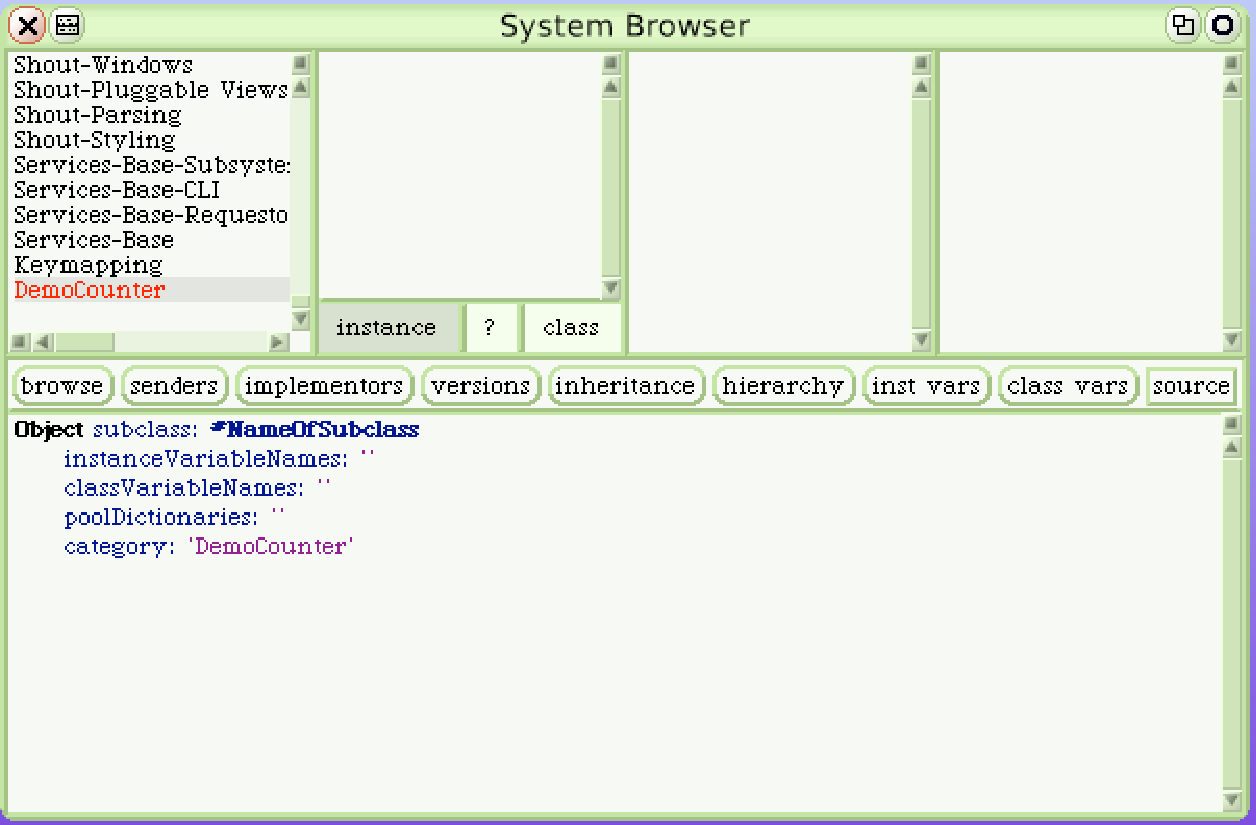
\includegraphics[scale=0.5]{nlesson3Fig4CategorySQ}}
\caption{Your category is created.} \label{fig:packageCreated}
\end{center}
\end{figure}}

Creating a class requires five steps. They consist basically of
editing the class definition template to specify the class you
want to create. \storespecific{\textit{Before you begin, make sure
that only the package \stc{DemoCounter} is selected.} (See
Figure ~\ref{fig:packageCreated})}

\begin{enumerate}
\item \textbf{Superclass Specification}. First, you should replace
the word \stc{NameOfSuperclass} with the word \stc{\vwspecific{Core.}Object}. Thus, you specify the superclass of the class you are creating. Note that this is not always the case that \stc{Object} is the superclass, since you may to inherit behavior from a class specializing already \stc{Object}.

\item \textbf{Class Name}. Next, you should fill in the name of
your class by replacing the word \stc{NameOfClass} with the
word \stc{SimpleCounter}. Take care that the name of the class
starts with a capital letter and that you do not remove the \#
sign in front of \stc{NameOfClass}.

\item \textbf{Instance Variable Specification}. Then, you should
fill in the names of the instance variables of this class. We need
one instance variable called \stc{value}. You add it by
replacing the words \textit{instVarName1} and
\textit{instVarName2} with the word \stc{value}. Take
care that you leave the string quotes!

\item \textbf{Class Variable Specification}. As we do not need any class variable make sure that the argument  for the class instance variables is an empty string (\ct{classInstanceVariableNames: ''}).

\item \textbf{Compilation}. That's it! We now have a filled-in
class definition for the class \ct{SimpleCounter}. To define it, we still have to \textbf{compile} it. Therefore,
select the \textbf{accept} option from the operate menu
(right-click button of the mouse). The class
\stc{SimpleCounter} is now compiled and immediately added to the system.
\end{enumerate}

As we are disciplined developers, we provide a comment to
\stc{SimpleCounter} class by clicking \textbf{Comment} \vwspecific{tab}\sqspecific{button} of
the class definition \vwspecific{(in the figure ~\ref{fig:packageCreated} the
\textbf{Comment} is highlighted)}. You can write the following
comment:

\begin{scode}
SimpleCounter is a concrete class which supports incrementing
and decrementing a counter.

Instance Variables:\\
value\tab \texttt{<}Integer\texttt{>}
\end{scode}

Select \textbf{accept} to store this class comment in the class.


\section{Defining protocols and methods}
In this part you will use the System Browser to learn how to add
protocols and methods.


\subsection{Creating and Testing Methods}
The class we have defined has one instance variable \ct{value}. You should
remember that in Smalltalk, everything is an object, that instance variables are private to the object and  that the only way to interact with an object is by sending messages to it.

Therefore, there is no other mechanism to access the instance variables from outside an object than sending a message to the object. What you can do is to define messages that return the value of the instance variable of a class. Such methods are called \textbf{accessors}, and it is a common practice to always define and use them. We start to create an accessor method for our instance variable \stc{value}.

Remember that every method belongs to a protocol. These protocols are just
a group of methods without any language semantics, but convey important
navigation information for the reader of your class. Although protocols
can have any name, Smalltalk programmers follow certain conventions for
naming these protocols. If you define a method and are not sure what
protocol it should be in, first go through existing code and try to
find a fitting name.


\paragraph{An important remark:} \textit{Accessors} can be defined in protocols
\ct{accessing} or \ct{private}.  Use the
\ct{accessing} protocol when a client object (like an
interface) really needs to access your data. Use \ct{private}
to clearly state that no client should use the accessor. This is
purely a convention. There is no way in Smalltalk to enforce
access rights like \emph{private} in C++ or Java.  To emphasize that objects are
not just data structure but provide services that are more
elaborated than just accessing data, put your accessors  in a
\ct{private} protocol. As a good practice, if you are not sure
then define your accessors in a \ct{private} protocol and
once some clients really need access, create
a protocol \ct{accessing} and move your methods there. Note
that this discussion does not seem to be very important in the
context of this specific simple example. However, this question is
central to the notion of object and encapsulation of the data. An
important side effect of this discussion is that you should always
ask yourself when you, as a client of an object, are using an
accessor if the object is really well defined and if it does not
need extra functionality.

\exercise Decide in which protocol you are going to put the accessor for \ct{value}. We now create the accessor method for the instance variable \ct{value}. Start by selecting the class
\ct{DemoCounter} in a browser, and make sure the \textbf{Instance}
\vwspecific{tab}\sqspecific{button} is selected \vwspecific{(in the figure ~\ref{fig:packageCreated}, the
\textbf{Instance} tab is in the middle of the window)}. Create a
new protocol clicking the right-button of the mouse on the pane of
methods categories, and choosing \ct{New}, and give a name. Select
the newly created protocol. Then in the bottom pane, the edit
field displays a method template laying out the default structure
of a method. Replace the template with the following method
definition:

\begin{scode}
value
     "return the current value of the value instance variable"

     ^value
\end{scode}

This defines a method called \ct{value}, taking no
arguments, having a method comment and returning the instance
variable \ct{value}. Then choose \textbf{accept} in the
operate menu (right button of the mouse) to compile the method. You
can now test your new method by typing and evaluating the next
expression in a Workspace, in the Transcript, or any text editor \ct{SimpleCounter new value}.

\vwspecific{To use a workspace, click on the 'noteblock' icon of the
launcher (last icon shown in Figure~\ref{fig:launcher}).}

\vwspecific{
\begin{figure}[htbp]
\begin{center}
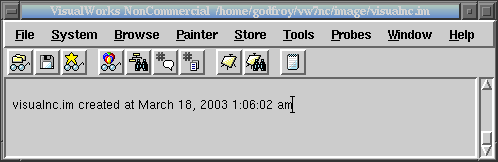
\includegraphics[scale=0.5]{nlesson1Fig1.png}
\caption{The Launcher of VisualWorks.}\label{fig:launcher}
\end{center}
\end{figure}}


This expression first creates a new instance of
\ct{SimpleCounter}, and then sends the message \ct{value} to it
and retrieves the current value of \ct{value}. This should return
\ct{nil} (the default value for noninitialised instance variables;
afterwards we will create instances where \ct{value} has a
reasonable default initialisation value).


\exercise  Another method that is normally used besides the
\textit{accessor} method is a so-called \textit{mutator} method.
Such a method is used to \emph{change} the value of an instance variable
from a client. For example, the next expression first creates a
new \ct{SimpleCounter} instance and then sets the value of
\ct{value} to 7:
\begin{scode}
SimpleCounter new value: 7
\end{scode}


This mutator method does not currently exist, so as an exercise
write the method \ct{value:} such that, when invoked on
an instance of \ct{SimpleCouter}, the \ct{value}
instance variable is set to the argument given to the message.
Test your method by typing and evaluating the expression above.

\exercise Implement the following methods in the protocol
\ct{operations}.

\begin{scode}
increment
    self value: self value + 1
decrement
    self value: self value - 1
\end{scode}

\exercise Implement the following methods in the protocol
\ct{printing}
\begin{scode}
printOn: aStream
    super printOn: aStream.
    aStream nextPutAll: ' with value: ',
    self  value printString.
    aStream cr.
\end{scode}

Now test the methods \ct{increment} and \ct{decrement} but pay
attention that the counter value is not initialized. Try:
\begin{scode}
SimpleCounter new value: 0; increment ; value.
\end{scode}
Note that the method \ct{printOn:} is used when you print an
object or click on \ct{self} in an inspector.

\vwspecific{
\subsection{Adding an instance creation method}
When we create a new instance of the class \ct{SimpleCounter}
using the message \ct{new}, we would like to obtain a well
initialized instance. To do so, we need to override the method
\ct{new} to add a call to an initialization method (invoking an
\ct{initialize} method is a very common practice! Ask for the
senders of \ct{initialize}). Notice that \ct{new} is always sent
to a class. This means that we have to define the new method on the
\emph{class side}, not on the \emph{instance side}. To define an instance creation method like the method
\ct{new} you should be on the class side, so you click on the
\textbf{Class} \vwspecific{tab}\sqspecific{button} (See in the figure ~\ref{fig:packageCreated},
the \textbf{Class} is situated in the same level as the
\textbf{Instance} \vwspecific{tab}\sqspecific{button}).

\exercise Define a new protocol called \ct{instance creation}, and
implement the method \ct{new} as follows:

%%bug with the \vwspecific macros all the text is flatten

\begin{alltt}
new
   "Create and return an initialized instance of SimpleCounter"
   \stBar newInstance \stBar
   newInstance := super new.
   newInstance initialize.
   \caret newInstance
\end{alltt}

This code returns a new and well initialized instance. We first
create a new instance by calling the normal creation method
(\ct{super new}), then we assign this new created instance
into the temporary variable called \ct{newInstance}. Then we
invoke the \ct{initialize} method on this new created instance
via the temporary variable and finally we return it.

Note that the previous method body is strictly equivalent to
the following one. Try to understand why they are equivalent.

\begin{scode}
new
   "Create and return an initialized instance of SimpleCounter"

   \caret super new initialize
\end{scode}
}

\subsection{Adding an instance initialization method}
Now we have to write an initialization method that sets a default
value to the \ct{value} instance variable. However, as
we mentioned the \ct{initialize} message is sent to the newly
created instance. This means that the \ct{initialize} method
should be defined at the instance side as any method that is sent
to an instance of \ct{SimpleCounter} like \ct{increment}
and \ct{decrement}. The \ct{initialize} method is responsible to set up the instance
variable default values.

Therefore at the instance side, you should create a protocol
\stc{initialize-release}, and create the following method (the body
of this method is left blank. Fill it in!).

\begin{scode}
initialize
   "set the initial value of the value to 0"
\end{scode}

\vwspecific{
\paragraph{Remark.} As we already mentioned, the \ct{initialize}
method is not automatically invoked by the method \ct{new}.
We had to override the method \ct{new} to call the
\ct{initialize} method. This is a weakness of the Smalltalk
libraries, so you should always check if the class that you are
creating inherits from a \ct{new} method that implements the
call to the \ct{initialize} method. It is a good practice to
add such a calling structure (\ct{new} calling
\ct{initialize}) in the root of the your class hierarchy. This
way you share the calling structure and are sure that the
\ct{initialize} method is always called for all your classes.
}

Now create a new instance of class \ct{SimpleCounter}. Is it
initialized by default? The following code should now work without
problem:

\begin{scode}
SimpleCounter new increment
\end{scode}

\subsection{Another instance creation method}
If you want to be sure that you have really understood the
distinction between instance and class methods, you should now define
a different instance creation method named \ct{withValue:}.
This method receives an integer as argument and returns an
instance of \ct{SimpleCounter} with the specified value. The
following expression should return 20.

\begin{scode}(SimpleCounter withValue: 19) increment ; value
\end{scode}

\hidden{
\paragraph{A Difficult Point}
Let us just think a bit! To create a new instance we said that we
should send messages (like \ct{new} and \ct{basicNew}) to
a class. For example to create an instance of
\ct{SimpleCounter} we sent \ct{new} to
\ct{SimpleCounter}. As the classes are also objects in
Smalltalk, they are instances of other classes that define the
structure and the behavior of classes. One of the classes that
represents classes as objects is \ct{Behavior}. Browse the
class \ct{Behavior}. In particular, \ct{Behavior} defines
the methods \ct{new} and \ct{basicNew} that are
responsible of creating new instances. If you did not redefine the
new message locally to the class of \ct{SimpleCounter}, when
you send the message \ct{new} to the class
\stc{SimpleCounter}, the new method executed is the one defined
in \ct{Behavior}. Try to understand why the methods \emph{new} and \emph{basicNew} are on the instance side on class \ct{Behavior} while they are on the class side of your class.}


\sd{Should add some Unit for VW too}
\squeakspecific{
\section{SUnit}
For the advanced ones, we suggest you to look at the videos and 
download the tutorial SUnit explained from
\ct{http://www.iam.unibe.ch/$\sim$ducasse/Books.html}. Then define a \ct{TestCase} with several tests for the \ct{SimpleCounter} class. To open the test runner execute
\begin{scode}
TestRunner open
\end{scode}}

\section{Saving your Work}
Several ways to save your work exist: You can
\begin{itemize}
\item Save the class by clicking on it and selecting the fileout menu item.
\item Use the Monticello browser to save a package
\end{itemize}

\squeaksourcespecific{You will use SqueakSource to save your work. Go to \ct{http://www.squeaksource.com/} and create a member account then register a new project. You get then an HTTP entry that refer to your project. Enter it as an HTTP repository in Monticello.}
\storespecific{To save our work, simply publish your package. This will open a dialog where you can give a comment, version numbers and blessing. After this is set, you can press Publish and your package will be stored in the database of Store. From then on, other people can load it from there, in the same way that you would use cvs or other multi-user versioning systems.
Saving the image is also a way to save your working environment, but publishing
it saves the code in the database. You can of course both publish your package (so that other people can load it, and that you can compare it with other versions, etc.) \emph{and} save your image (so that next time that you start your image you are in the same working environment).}
\parcelspecific{To save our work, simply \textit{Publish as Parcel} your package. Normally each option should fit with your need. By pressing \textit{Publish} two files will be created DemoCounter.pcl and DemoCounter.pst\footnote{DemoCounter.pcl contains only the binary code, whereas the .pst file contains only the source code}.After starting a new image, you can load back your application by choosing \textit{Load Parcel Named} in the menu \textit{Tools}; a dialog box will popup for entering a regular expression, just enter \stc{Demo*}.}

\ifx\wholebook\relax\else\end{document}\fi

\end{document}
